\subsubsection{Synthesis of homoserine lactone-ciprofloxacin triazole conjugates with cleavable linkers\label{sec:cleavable}}

%To address this a sceond set of conjugates were prepared in collaboration with Professor Eddy Sotelo, a visiting academic in the Spring group. 
%
%OR:
%
%you could go with something like: in parallel with the perpetration of xxx, a second ciprofloxicin alkyne was prepared by Eddie Soleto. and do the bio together. just be more positive nad view it as a collaboration, just because yours didn't work doesnt mean they didnt contribute to the knowledge that you need the biocleavable linker. In fact. he needed you and your azides! :) 

In addition to the conjugates shown in the previous section, a further collection was synthesised in collaboration with Professor Eddy Sotelo, a visiting researcher in the Spring group. Professor Sotelo synthesised two alkyne-linked ciprofloxacin derivatives \compound{cmpd:Y4HCip} and \compound{cmpd:Y4MeCip} (see \ref{fig:cleavable_Ys}), both with cleavable linkers (see \ref{sec:cleavable_intro}). 

\begin{figure}[H]
	\begin{center}
		\schemeref[Y4HCip]{cmpd:Y4HCip}
		\schemeref[Y4MeCip]{cmpd:Y4MeCip}
		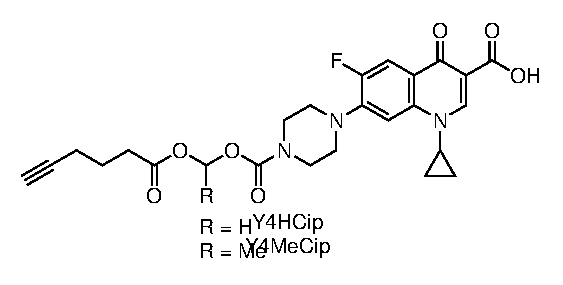
\includegraphics[scale=1]{cleavable_Ys}
		\caption{
			The cleavable alkyne-Cip derivatives synthesised by Professor Sotelo.
			\label{fig:cleavable_Ys}}
	\end{center}
\end{figure}

Professor Sotelo then performed click reactions using the AHL azide derivatives \compound{cmpd:HL2N3}, \compound{cmpd:HL4N3} and \compound{cmpd:HL6N3} synthesised in \ref{sec:HSLs} to form a new set of conjugates to add to the library (see \ref{fig:cleavable_finals}). It was hoped that these conjugates would enter the cell and then be cleaved by esterases to release ciprofloxcin (see \ref{sec:cleavable_intro}).

\begin{figure}[H]
	\begin{center}
		\schemeref[HL2THCip]{cmpd:HL2THCip}
		\schemeref[HL4THCip]{cmpd:HL4THCip}
		\schemeref[HL6THCip]{cmpd:HL6THCip}
		\schemeref[HL2TMeCip]{cmpd:HL2TMeCip}
		\schemeref[HL4TMeCip]{cmpd:HL4TMeCip}
		\schemeref[HL6TMeCip]{cmpd:HL6TMeCip}
		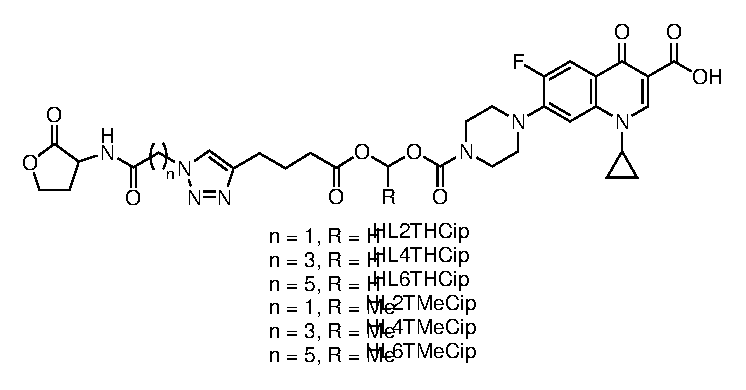
\includegraphics[scale=1]{cleavable_finals}
		\caption{
			The cleavable HSL-Cip triazole conjugates synthesised by Professor Sotelo.
			\label{fig:cleavable_finals}}
	\end{center}
\end{figure}

Two control compounds \compound{cmpd:BnTHCip} and \compound{cmpd:BnTMeCip} with benzyl head groups were also produced by Professor Sotelo (see \ref{fig:cleavable_controls}). It was hoped that these would show whether the AHL head group is required for activity.

\begin{figure}[H]
	\begin{center}
		\schemeref[BnTHCip]{cmpd:BnTHCip}
		\schemeref[BnTMeCip]{cmpd:BnTMeCip}
		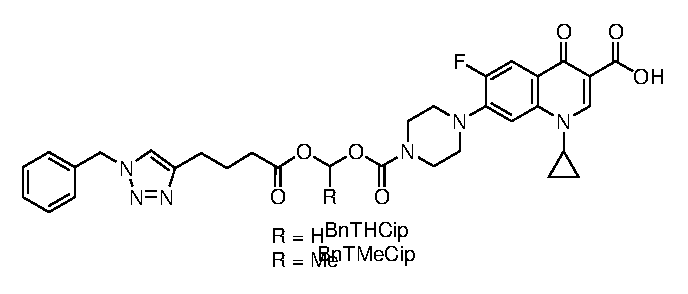
\includegraphics[scale=1]{cleavable_controls}
		\caption{
			The cleavable Bn-Cip triazole conjugates \compound{cmpd:BnTHCip} and \compound{cmpd:BnTMeCip} synthesised by Professor Sotelo.
			\label{fig:cleavable_controls}}
	\end{center}
\end{figure}


